\documentclass{report}
\usepackage[T1]{fontenc} % Fontes T1
\usepackage[utf8]{inputenc} % Input UTF8
\usepackage[backend=biber, style=ieee]{biblatex} % para usar bibliografia
\usepackage{csquotes}
\usepackage[portuguese]{babel} %Usar língua portuguesa
\usepackage{blindtext} % Gerar texto automaticamente
\usepackage[printonlyused]{acronym}
\usepackage{hyperref} % para autoref
\usepackage{graphicx}

\bibliography{bibliografia}


\begin{document}
%%
% Definições
%
\def\titulo{Adivinha o Número Secreto}
\def\data{30/05/2020}
\def\autores{Mauro Marques Canhão Filho, Patricia Rafaela da Rocha Cardoso }
\def\autorescontactos{(103411) mauro.filho@ua.pt, (103243) patriciarcardoso@ua.pt}
\def\versao{1.0}
\def\departamento{Departamento de Eletrônica, Telecomunicações e Informática (DETI)}
\def\empresa{Universidade de Aveiro}
\def\logotipo{ua.pdf}
%
%%%%%% CAPA %%%%%%
%
\renewcommand{\contentsname}{Índice}
\begin{titlepage}

\begin{center}
%
\vspace*{50mm}
%
{\Huge \titulo}\\ 
%
\vspace{10mm}
%
{\Large \empresa}\\
%
\vspace{10mm}
%
{\LARGE \autores}\\ 
%
\vspace{30mm}
%
\begin{figure}[h]
\center
\includegraphics{\logotipo}
\end{figure}
%
\vspace{30mm}
\end{center}
%
\begin{flushright}
\versao
\end{flushright}
\end{titlepage}

%%  Página de Título %%
\title{%
{\Huge\textbf{\titulo}}\\
{\Large \departamento\\ \empresa}
}
%
\author{%
    \autores \\
    \autorescontactos
}
%
\date{\data}
%
\maketitle

\pagenumbering{roman}

%%%%%% RESUMO %%%%%%
\begin{abstract}
Este relatório tem como objetivo descrever a implementação e a intereção entre um servidor e um ou mais clientes. Para isso, será detalhadamente apresentado o funcionamento/criação de um jogo. O jogo consiste em o cliente adivinhar um número inteiro aleatório entre 0 e 100, o número secreto, gerado aleatoriamente pelo servidor.
\end{abstract}

\tableofcontents
% \listoftables     % descomentar se necessário
% \listoffigures    % descomentar se necessário


%%%%%%%%%%%%%%%%%%%%%%%%%%%%%%%
\clearpage
\pagenumbering{arabic}

%%%%%%%%%%%%%%%%%%%%%%%%%%%%%%%%
\chapter{Introdução}
\label{chap.introducao}
O objetivo deste trabalho é explicar,enumerar e descrever o desenvolvimento e funcionamento de um servidor que suporte a geração de um número inteiro aleatório (entre 0 e 100), o número secreto, bem como o número máximo de tentativas (entre 10 e 30) concedidas para o adivinhar. E um cliente que permita adivinhar esse número secreto. Ou seja um jogo de adivinha o número secreto.
O servidor nunca deverá aceitar dois clientes com a mesma identificação a jogar simultaneamente e deverá criar e atualizar um ficheiro designado por report.csv onde vai escrevendo os resultados dos diversos clientes quando estes terminam o jogo. O cliente pode desistir em qualquer altura e o jogo acaba quando ele adivinha o número secreto ou quando esgota o número máximo de tentativas que dispunha para jogar. Caso o cliente exceda o número de jogadas de que dispunha o jogo será considerado sem sucesso mesmo que ele tenha adivinhado o número. Quando o jogo acaba corretamente o cliente deve escrever no monitor uma mensagem a indicar se adivinhou ou não o número secreto e quantas jogadas efectuou. Por sua vez o servidor acrescenta ao ficheiro a informação relativa ao jogo: cliente; número secreto; número máximo de jogadas; número de jogadas efectuadas; e o resultado obtido pelo cliente (desistência ou sucessso ou insucessso).

\chapter{Metodologia}
\label{chap.metodologia}
Neste capítulo será detalhadamente descrito o algoritmo e o funcionamento do progama servidor e do programa cliente bem como a implementação dos testes funcionais e unitários.

O programa servidor consiste em gerar aleatoriamente um número entre 0 e 100 e um número máximo de tentativas entre 10 e 30 para o adivinhar. 
\begin{figure}[h]
	\centering
	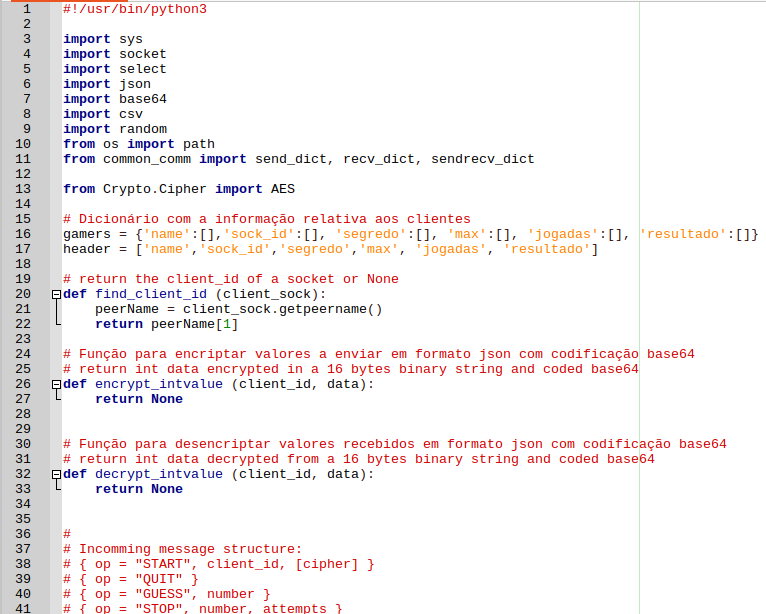
\includegraphics[scale=0.58]{server1}	
	\caption{Programa Servidor}
\end{figure}


\chapter{Resultados}
\label{chap.resultados}

\chapter{Análise}
\label{chap.analise}


\chapter{Conclusões}
\label{chap.conclusao}

\chapter*{Contribuições dos autores}


%%%%%%%%%%%%%%%%%%%%%%%%%%%%%%%%%
\chapter*{Acrónimos}


%%%%%%%%%%%%%%%%%%%%%%%%%%%%%%%%%
\printbibliography

\end{document}
